\documentclass[]{article}
\usepackage{lmodern}
\usepackage{amssymb,amsmath}
\usepackage{bm}
\usepackage{soul}
\usepackage[color=yellow]{todonotes}
\usepackage{ifxetex,ifluatex}
\usepackage{fixltx2e} % provides \textsubscript
\ifnum 0\ifxetex 1\fi\ifluatex 1\fi=0 % if pdftex
  \usepackage[T1]{fontenc}
  \usepackage[utf8]{inputenc}
\else % if luatex or xelatex
  \ifxetex
    \usepackage{mathspec}
  \else
    \usepackage{fontspec}
  \fi
  \defaultfontfeatures{Ligatures=TeX,Scale=MatchLowercase}
\fi
% use upquote if available, for straight quotes in verbatim environments
\IfFileExists{upquote.sty}{\usepackage{upquote}}{}
% use microtype if available
\IfFileExists{microtype.sty}{%
\usepackage{microtype}
\UseMicrotypeSet[protrusion]{basicmath} % disable protrusion for tt fonts
}{}
\usepackage[margin=1in]{geometry}
\usepackage{hyperref}
\hypersetup{unicode=true,
            pdftitle={11 Dynamic models and their simulation by Euler's method},
            pdfauthor={Edward Ionides},
            pdfborder={0 0 0},
            breaklinks=true}
\urlstyle{same}  % don't use monospace font for urls
\usepackage{color}
\usepackage{fancyvrb}
\newcommand{\VerbBar}{|}
\newcommand{\VERB}{\Verb[commandchars=\\\{\}]}
\DefineVerbatimEnvironment{Highlighting}{Verbatim}{commandchars=\\\{\}}
% Add ',fontsize=\small' for more characters per line
\usepackage{framed}
\definecolor{shadecolor}{RGB}{248,248,248}
\newenvironment{Shaded}{\begin{snugshade}}{\end{snugshade}}
\newcommand{\KeywordTok}[1]{\textcolor[rgb]{0.13,0.29,0.53}{\textbf{#1}}}
\newcommand{\DataTypeTok}[1]{\textcolor[rgb]{0.13,0.29,0.53}{#1}}
\newcommand{\DecValTok}[1]{\textcolor[rgb]{0.00,0.00,0.81}{#1}}
\newcommand{\BaseNTok}[1]{\textcolor[rgb]{0.00,0.00,0.81}{#1}}
\newcommand{\FloatTok}[1]{\textcolor[rgb]{0.00,0.00,0.81}{#1}}
\newcommand{\ConstantTok}[1]{\textcolor[rgb]{0.00,0.00,0.00}{#1}}
\newcommand{\CharTok}[1]{\textcolor[rgb]{0.31,0.60,0.02}{#1}}
\newcommand{\SpecialCharTok}[1]{\textcolor[rgb]{0.00,0.00,0.00}{#1}}
\newcommand{\StringTok}[1]{\textcolor[rgb]{0.31,0.60,0.02}{#1}}
\newcommand{\VerbatimStringTok}[1]{\textcolor[rgb]{0.31,0.60,0.02}{#1}}
\newcommand{\SpecialStringTok}[1]{\textcolor[rgb]{0.31,0.60,0.02}{#1}}
\newcommand{\ImportTok}[1]{#1}
\newcommand{\CommentTok}[1]{\textcolor[rgb]{0.56,0.35,0.01}{\textit{#1}}}
\newcommand{\DocumentationTok}[1]{\textcolor[rgb]{0.56,0.35,0.01}{\textbf{\textit{#1}}}}
\newcommand{\AnnotationTok}[1]{\textcolor[rgb]{0.56,0.35,0.01}{\textbf{\textit{#1}}}}
\newcommand{\CommentVarTok}[1]{\textcolor[rgb]{0.56,0.35,0.01}{\textbf{\textit{#1}}}}
\newcommand{\OtherTok}[1]{\textcolor[rgb]{0.56,0.35,0.01}{#1}}
\newcommand{\FunctionTok}[1]{\textcolor[rgb]{0.00,0.00,0.00}{#1}}
\newcommand{\VariableTok}[1]{\textcolor[rgb]{0.00,0.00,0.00}{#1}}
\newcommand{\ControlFlowTok}[1]{\textcolor[rgb]{0.13,0.29,0.53}{\textbf{#1}}}
\newcommand{\OperatorTok}[1]{\textcolor[rgb]{0.81,0.36,0.00}{\textbf{#1}}}
\newcommand{\BuiltInTok}[1]{#1}
\newcommand{\ExtensionTok}[1]{#1}
\newcommand{\PreprocessorTok}[1]{\textcolor[rgb]{0.56,0.35,0.01}{\textit{#1}}}
\newcommand{\AttributeTok}[1]{\textcolor[rgb]{0.77,0.63,0.00}{#1}}
\newcommand{\RegionMarkerTok}[1]{#1}
\newcommand{\InformationTok}[1]{\textcolor[rgb]{0.56,0.35,0.01}{\textbf{\textit{#1}}}}
\newcommand{\WarningTok}[1]{\textcolor[rgb]{0.56,0.35,0.01}{\textbf{\textit{#1}}}}
\newcommand{\AlertTok}[1]{\textcolor[rgb]{0.94,0.16,0.16}{#1}}
\newcommand{\ErrorTok}[1]{\textcolor[rgb]{0.64,0.00,0.00}{\textbf{#1}}}
\newcommand{\NormalTok}[1]{#1}
\usepackage{graphicx,grffile}
\makeatletter
\def\maxwidth{\ifdim\Gin@nat@width>\linewidth\linewidth\else\Gin@nat@width\fi}
\def\maxheight{\ifdim\Gin@nat@height>\textheight\textheight\else\Gin@nat@height\fi}
\makeatother
% Scale images if necessary, so that they will not overflow the page
% margins by default, and it is still possible to overwrite the defaults
% using explicit options in \includegraphics[width, height, ...]{}
\setkeys{Gin}{width=\maxwidth,height=\maxheight,keepaspectratio}
\IfFileExists{parskip.sty}{%
\usepackage{parskip}
}{% else
\setlength{\parindent}{0pt}
\setlength{\parskip}{6pt plus 2pt minus 1pt}
}
\setlength{\emergencystretch}{3em}  % prevent overfull lines
\providecommand{\tightlist}{%
  \setlength{\itemsep}{0pt}\setlength{\parskip}{0pt}}
%\setcounter{secnumdepth}{0}
\setcounter{section}{11}
% Redefines (sub)paragraphs to behave more like sections
\ifx\paragraph\undefined\else
\let\oldparagraph\paragraph
\renewcommand{\paragraph}[1]{\oldparagraph{#1}\mbox{}}
\fi
\ifx\subparagraph\undefined\else
\let\oldsubparagraph\subparagraph
\renewcommand{\subparagraph}[1]{\oldsubparagraph{#1}\mbox{}}
\fi

%%% Use protect on footnotes to avoid problems with footnotes in titles
\let\rmarkdownfootnote\footnote%
\def\footnote{\protect\rmarkdownfootnote}

%%% Change title format to be more compact
\usepackage{titling}

% Create subtitle command for use in maketitle
\newcommand{\subtitle}[1]{
  \posttitle{
    \begin{center}\large#1\end{center}
    }
}

\setlength{\droptitle}{-2em}
  \title{11. Dynamic models and their simulation by Euler's method}
  \pretitle{\vspace{\droptitle}\centering\huge}
  \posttitle{\par}
  \author{Edward Ionides}
  \preauthor{\centering\large\emph}
  \postauthor{\par}
  \predate{\centering\large\emph}
  \postdate{\par}
  \date{3/25/2018}


\begin{document}
\maketitle

{
\setcounter{tocdepth}{2}
\tableofcontents
}
\newcommand\prob{\mathbb{P}}
\newcommand\E{\mathbb{E}}
\newcommand\cov{\mathrm{Cov}}
\newcommand\loglik{\ell}
\newcommand\R{\mathbb{R}}
\newcommand\data[1]{#1^*}
\newcommand\params{\, ; \,}
\newcommand\transpose{\scriptsize{T}}
\newcommand\eqspace{\quad\quad}
\newcommand\myeq[1]{\eqspace \displaystyle #1}
\newcommand\lik{\mathscr{L}}
\newcommand\profileloglik[1]{\ell^\mathrm{profile}_#1}
\newcommand\ar{\phi}
\newcommand\ma{\psi}
\newcommand\AR{\Phi}
\newcommand\MA{\Psi}
\newcommand\ev{u}
\newcommand\given{{\, | \,}}
\newcommand\equals{{=\,}}
\newcommand\matA{\mathbb{A}}
\newcommand\matB{\mathbb{B}}
\newcommand\matH{\mathbb{H}}
\newcommand\covmatX{\mathbb{U}}
\newcommand\covmatY{\mathbb{V}}


\begin{center}\rule{0.5\linewidth}{\linethickness}\end{center}

\newcommand\expect[1]{\mathbb{E}\left[{#1}\right]}
\newcommand\var[1]{\mathrm{Var}\left[{#1}\right]}
\newcommand\dist[2]{\mathrm{#1}\left(#2\right)}
\newcommand\dlta{\Delta}


Produced with R version 3.4.3 and \textbf{pomp} version 1.16.

\begin{center}\rule{0.5\linewidth}{\linethickness}\end{center}

Objectives

This chapter develops a general class of \hl{dynamic models with particular
relevance for biological systems}. We have the following goals:

\begin{enumerate}
\def\labelenumi{\arabic{enumi}.}
\item
  Dynamic systems can often be represented in terms of \emph{flows}
  between \emph{compartments}. We will develop the concept of a
  \emph{compartment model} for which we \hl{specify \emph{rates} for the
  flows between compartments.}
\item
  We develop deterministic and stochastic interpretations of a
  compartment model.
\item
  We introduce Euler's method to simulate from dynamic models, and we
  apply it to both deterministic and stochastic compartment models.
\end{enumerate}

\begin{center}\rule{0.5\linewidth}{\linethickness}\end{center}

\begin{center}\rule{0.5\linewidth}{\linethickness}\end{center}

\subsection{Compartment models}\label{compartment-models}

\begin{itemize}
\item
  A \hl{\textbf{compartment model} is a model associated with a \textbf{flow
  diagram}} specifying how objects move between categories, called
  \textbf{compartments}.
\item
  It is often useful to represent systems by \textbf{flow diagrams}. We
  will need equations to specify formally what the flow diagram means.
\item
  One major applications of compartment models is
  \href{https://en.wikipedia.org/wiki/Pharmacokinetics}{pharmacokinetics},
  the study of how pharmacological drugs enter the body, move between
  organs, metabolize, and leave. The compartments may be the organs; the
  flow is movement of the drug and its metabolites between organs.
\item
  Another major application of compartment models is
  \href{https://en.wikipedia.org/wiki/Compartmental_models_in_epidemiology}{epidemiology}.
  Compartments are groups of people; the flow is the movement of an
  infectious disease through the population.
\end{itemize}

\begin{center}\rule{0.5\linewidth}{\linethickness}\end{center}

\begin{center}\rule{0.5\linewidth}{\linethickness}\end{center}

\subsection{Compartment models in epidemiology: the SIR model and its
generalizations}\label{compartment-models-in-epidemiology-the-sir-model-and-its-generalizations}

We will develop deterministic and stochastic representations of a
\hl{susceptible-infected-recovered (SIR) system}, a fundamental class of
\hl{models for disease transmission dynamics}. We will do this using notation
which generalizes to more complex systems
\href{http://dept.stat.lsa.umich.edu/~ionides/pubs/breto09.pdf}{{[}@breto09{]}}.

\hypertarget{htmlwidget-c91d56e95a6c9d1fe971}{}

$$S\longrightarrow I\longrightarrow R $$

\(S = \text{susceptible}\)\\
\(I = \text{infected and infectious}\)\\
\(R = \text{recovered and/or removed}\)

\begin{itemize}
\item
  We suppose that each arrow has an associated rate, so here there is a
  rate \(\mu_{SI}(t)\) at which individuals in \(S\) transition to
  \(I\), and \(\mu_{IR}\) at which individuals in \(I\) transition to
  \(R\).
  
  \todo[inline]{Here, $\mu_{SI}(t)$ have units of $t^{-1}$ --  infections per unit time (infections are dimensionless, i.e. counts don't have dimensions). Thus, $\beta$ has units $t^{-1}$ as well.}
  
\item
  To \hl{account for demography (births/deaths/immigration/emmigration)} we
  allow the possibility of a source and sink compartment, which is not
  usually represented on the flow diagram. We write
  \hl{$\mu_{{\small{\bullet}}S}$ for a rate of births into $S$}, and
  denote mortality rates by $\mu_{S{\small\bullet}}$,
  $\mu_{I{\small\bullet}}$, $\mu_{R{\small\bullet}}$.
\item
  The rates may be either constant or varying. In particular, for a
  simple SIR model, the recovery rate \(\mu_{IR}\) is a constant but the
  infection rate has the time-varying form
  \[\mu_{SI}(t)=\beta \, I(t),\] with \(\beta\) being the \emph{contact
  rate}. Now, for the simplest SIR model, ignoring demography, we set
  \[ \mu_{{\small{\bullet}}S}=\mu_{S{\small{\bullet}}}=\mu_{I{\small{\bullet}}}=\mu_{R{\small{\bullet}}}=0.\]
\item
  To develop a systemtic notation, it turns out to be convenient to keep
  track of the flows between compartments as well as the number of
  individuals in each compartment. Let \[N_{SI}(t)\] count the \hl{number of
  individuals who have transitioned from $S$ to $I$ by time $t$}.
  We say that \(N_{SI}(t)\) is a \emph{counting process}. A similarly
  constructed process \[N_{IR}(t)\] counts individuals transitioning
  from \(I\) to \(R\). To include demography, we could keep track of
  birth and death events by the counting processes
  \(N_{{\small{\bullet}} S}(t)\), \(N_{S{\small{\bullet}}}(t)\),
  \(N_{I{\small{\bullet}}}(t)\), \(N_{R{\small{\bullet}}}(t)\).
\item
  For discrete population compartment models, the flow counting
  processes are non-decreasing and integer valued.
\item
  For continuous population compartment models, the flow counting
  processes are non-decreasing and real valued.
\item
  The \hl{numbers of people in each compartment} can be computed via these
  counting processes. Ignoring demography, we have:
  \[\begin{array}{lcl} 
  S(t)&=& S(0) - N_{SI}(t)
  \\
  I(t)&=& I(0) + N_{SI}(t) - N_{IR}(t)
  \\
  R(t) &=& R(0) + N_{IR}(t)
  \end{array}\]
\item
  These equations represent something like \emph{conservation of mass},
  or \emph{what goes in must come out}.
\end{itemize}

\begin{center}\rule{0.5\linewidth}{\linethickness}\end{center}

\begin{center}\rule{0.5\linewidth}{\linethickness}\end{center}

\subsection{\texorpdfstring{The \emph{ordinary differential equation}
(ODE) interpretation of the SIR
model}{The ordinary differential equation (ODE) interpretation of the SIR model}}\label{the-ordinary-differential-equation-ode-interpretation-of-the-sir-model}

Together with initial conditions specifying \(S(0)\), \(I(0)\) and
\(R(0)\), we just need to write down ODEs for the flow counting
processes. These are, \[ dN_{SI}/dt = \mu_{SI}(t) \, S(t),\]
\[ dN_{IR}/dt = \mu_{IR}\, I(t).\]

\begin{center}\rule{0.5\linewidth}{\linethickness}\end{center}

\begin{center}\rule{0.5\linewidth}{\linethickness}\end{center}

\subsection{The simple continuous-time Markov chain interpretation of
the SIR
model}\label{the-simple-continuous-time-markov-chain-interpretation-of-the-sir-model}

\begin{itemize}
\item
  \hl{Continuous-time Markov chains} are the basic tool for building discrete
  population epidemic models.
\item
  Recall that a \emph{Markov chain} is a discrete-valued stochastic
  process with the \emph{Markov property}: the future evolution of the
  process depends only on the current state.
\item
  Surprisingly many models have this Markov property. If all important
  variables are included in the state of the system, then the Markov
  property appears automatically.
\item
  The Markov property lets us specify a model by the transition
  probabilities on small intervals (together with the initial
  conditions). For the SIR model, we have
\end{itemize}

\[\begin{array}{lcl}
\prob\big[N_{SI}(t+\delta)\equals N_{SI}(t)+1\big] &=& \mu_{SI}(t) \, S(t) \delta + o(\delta)
\\
\prob\big[N_{SI}(t+\delta)\equals N_{SI}(t)\big] &=& 1-\mu_{SI}(t) \, S(t) \delta + o(\delta)
\\
\prob\big[N_{IR}(t+\delta)\equals N_{IR}(t)+1\big] &=& \mu_{IR} \, I(t) \delta + o(\delta)
\\
\prob\big[N_{IR}(t+\delta)\equals N_{IR}(t)\big] &=& 1-\mu_{IR}(t) \, I(t) \delta + o(\delta)
\end{array}\]

\begin{itemize}
\tightlist
\item
  Here, \hl{we are using}
  \href{https://en.wikipedia.org/wiki/Big_O_notation\#Little-o_notation}{little
  $o$ notation}\hl{.} We write \[ h(\delta)=o(\delta)\] to mean
  \[ \lim_{\delta\to 0} \frac{h(\delta)}{\delta} = 0.\]
\end{itemize}

\begin{center}\rule{0.5\linewidth}{\linethickness}\end{center}

\begin{center}\rule{0.5\linewidth}{\linethickness}\end{center}

\subsubsection{\texorpdfstring{Question: What is the link between little
\(o\) notation and the
derivative?}{Question: What is the link between little o notation and the derivative?}}\label{question-what-is-the-link-between-little-o-notation-and-the-derivative}

\begin{itemize}
\item
  Explain why \[f(x+\delta)=f(x)+ \delta g(x) + o(\delta)\] is the same
  statement as \[ \frac{df}{dx} = g(x).\]
\item
  What considerations might help you choose which of these notations to
  use?
\end{itemize}

\begin{center}\rule{0.5\linewidth}{\linethickness}\end{center}

\begin{center}\rule{0.5\linewidth}{\linethickness}\end{center}

\subsection{Exercises}\label{exercises}

\subsubsection{From Markov chain to ODE}\label{from-markov-chain-to-ode}

Find the expected value of \(N_{SI}(t+\delta)-N_{SI}(t)\) and
\(N_{IR}(t+\delta)-N_{IR}(t)\) given the current state, \(S(t)\),
\(I(t)\) and \(R(t)\). Take the limit as \(\delta\to 0\) and show that
this gives the ODE model.

\begin{itemize}
\item
  A \emph{simple} counting process is one which cannot count more than
  one event at a time
  (\href{https://en.wikipedia.org/wiki/Point_process}{Wikipedia:
  Point\_process}). Thus, in a technical sense, the SIR Markov chain
  model we have written is simple. One may want to model the extra
  randomness resulting from multiple simultaneous events: someone
  sneezing in a bus; large gatherings at football matches; etc. This
  extra randomness may even be critical to match the variability in
  data.
\item
  Later in the course, we may see situations where this extra randomness
  plays an important role. Setting up the model using counting
  processes, as we have done here, turns out to be useful for this.
\end{itemize}

\begin{center}\rule{0.5\linewidth}{\linethickness}\end{center}

\begin{center}\rule{0.5\linewidth}{\linethickness}\end{center}

\subsection{Euler's method for ordinary differential equations
(ODEs)}\label{eulers-method-for-ordinary-differential-equations-odes}

\begin{itemize}
\item
  \href{https://en.wikipedia.org/wiki/Leonhard_Euler}{Euler} took the
  following approach to numeric solution of an ODE:

  \begin{itemize}
  \tightlist
  \item
    He wanted investigate an ODE \[dx/dt = h(x)\] with an initial
    condition \(x(0)\). He supposed this ODE has some true solution
    \(x(t)\) which could not be worked out analytically. He therefore
    wished to \hl{approximate $x(t)$ numerically.}
  \item
    He initialized the numerical solution at the known starting value,
    \[\tilde x(0)=x(0).\] Then, for \(k=1,2,\dots\), he supposed that
    the gradient \(dx/dt\) is approximately constant over the small time
    interval \(k\delta\le t\le (k+1)\delta\). Therefore, he defined
    \[\tilde x\big( \,(k+1)\delta\,\big) = \tilde x( k\delta) + \delta \, h\big(\, \tilde x(k\delta)\,\big).\]
  \end{itemize}
\item
  This only defines \(\tilde x(t)\) when \(t\) is a multiple of
  \(\delta\), but let's suppose \(\tilde x(t)\) is constant between
  these discrete times.
\item
  We now have a numerical scheme, stepping forwards in time increments
  of size \(\delta\), that can be readily evaluated by computer (or by
  hand, if you are Euler).
\item
  \href{https://en.wikipedia.org/wiki/Euler_method}{Mathematical
  analysis of Euler's method} says that, as long as the function
  \(h(x)\) is not too exotic, then \(x(t)\) is well approximated by
  \(\tilde x(t)\) when the discretization time-step, \(\delta\), is
  sufficiently small.
\item
  Euler's method is not the only numerical scheme to solve ODEs. More
  advanced schemes have better convergence properties, meaning that the
  numerical approximation is closer to \(x(t)\). However, there are 3
  reasons we choose to lean heavily on Euler's method:
\end{itemize}

\begin{enumerate}
\def\labelenumi{\arabic{enumi}.}
\item
  Euler's method is the simplest (following the KISS principle).
\item
  Euler's method extends naturally to stochastic models, both
  continuous-time Markov chains models and stochastic differential
  equation (SDE) models.
\item
  Close approximation of the numerical solutions to a continuous-time
  model is less important than it may at first appear, a topic worth
  further discussion\ldots{}
\end{enumerate}

\begin{center}\rule{0.5\linewidth}{\linethickness}\end{center}

\begin{center}\rule{0.5\linewidth}{\linethickness}\end{center}

\subsection{Some comments on using continuous-time models and
discretized
approximations}\label{some-comments-on-using-continuous-time-models-and-discretized-approximations}

\begin{itemize}
\item
  In some physical and engineering situations, a system follows an ODE
  model closely. For example, Newton's laws provide a very good
  approximation to the motions of celestial bodies.
\item
  In many biological situations, ODE models only become close
  mathematical approximations to reality at reasonably large scale. On
  small temporal scales, models cannot usually capture the full scope of
  biological variation and biological complexity.
\item
  If we are going to expect substantial error in using \(x(t)\) to model
  a biological system, maybe the numerical solution \(\tilde x(t)\)
  represents the system being modeled as well as \(x(t)\) does.
\item
  If our model fitting, model investigation, and final conclusions are
  all based on our numerical solution \(\tilde x(t)\) (i.e., we are
  sticking entirely to simulation-based methods) then we are most
  immediately concerned with how well \(\tilde x(t)\) describes the
  system of interest. \(\tilde x(t)\) becomes more important than the
  original model, \(x(t)\).
\item
  When following this perspective, it is important that the scientists
  fully describe the numerical model \(\tilde x(t)\). The main advantage
  of the continuous-time model \(x(t)\) is then that it gives a succinct
  way to describe how \(\tilde x(t)\) was constructed.
\item
  All numerical methods are, ultimately, discretizations.
  Epidemiologically, setting \(\delta\) to be a day, or an hour, can be
  quite different from setting \(\delta\) to be two weeks or a month.
  For continuous-time modeling, we still require that \(\delta\) is
  small compared to the timescale of the process being modeled, and the
  choice of \(\delta\) does not play an explicit role in the
  interpretation of the model.
\item
  Putting more emphasis on the scientific role of the numerical solution
  itself reminds you that the numerical solution has to do more than
  approximate a target model in some asymptotic sense: the numerical
  solution should be a sensible model in its own right.
\end{itemize}

\begin{center}\rule{0.5\linewidth}{\linethickness}\end{center}

\begin{center}\rule{0.5\linewidth}{\linethickness}\end{center}

\subsection{Euler's method for a discrete SIR
model}\label{eulers-method-for-a-discrete-sir-model}

\begin{itemize}
\tightlist
\item
  Recall the simple continuous-time Markov chain interpretation of the
  SIR model without demography:
\end{itemize}

\[\begin{array}{lcl}
\prob\big[N_{SI}(t+\delta)\equals N_{SI}(t)+1\big] &=& \mu_{SI}(t) \, S(t) \delta + o(\delta),
\\
\prob\big[N_{IR}(t+\delta)\equals N_{IR}(t)+1\big] &=& \mu_{IR} \, I(t) \delta + o(\delta).
\end{array}\]

\begin{itemize}
\item
  We look for a numerical solution with state variables
  \(\tilde S(k\delta)\), \(\tilde I(k\delta)\), \(\tilde R(k\delta)\).
\item
  The counting processes for the flows between compartments are
  \(\tilde N_{SI}(t)\) and \(\tilde N_{IR}(t)\). The counting processes
  are related to the numbers of individuals in the compartments by the
  same flow equations we had before: \[\begin{array}{lcl} 
  \tilde S(k\delta)&=& S(0) - \tilde N_{SI}(k\delta)
  \\
  \tilde I(k\delta)&=& I(0) + \tilde N_{SI}(k\delta) - \tilde N_{IR}(k\delta)
  \\
  \tilde R(k\delta) &=& R(0) + \tilde N_{IR}(k\delta)
  \end{array}\]
\item
  Let's focus on a numerical solution to \(N_{SI}(t)\), since the same
  methods can also be applied to \(N_{IR}(t)\).
\item
  Here are three possibilities, defining a process at times
  \(t=k\delta\) for all integer \(k\) and some fixed \(\delta>0\).
\end{itemize}

\begin{enumerate}
\def\labelenumi{\arabic{enumi}.}
\tightlist
\item
  A Poisson approximation.
  \[\tilde N_{SI}(t+\delta)= \tilde N_{SI}(t) + \mathrm{Poisson}\big[\mu_{SI}\big(\tilde I(t)\big) \, \tilde S(t) \,\delta\big],\]
  where \(\mathrm{Poisson}(\mu)\) is a Poisson random variable with mean
  \(\mu\) and \[\mu_{SI}\big(\tilde I(t)\big) = \beta\, \tilde I(t).\]
\end{enumerate}

\begin{enumerate}
\def\labelenumi{\arabic{enumi}.}
\setcounter{enumi}{1}
\tightlist
\item
  A binomial approximation with transition probabilities approximated by
  rate times time.
  \[\tilde N_{SI}(t+\delta) = \tilde N_{SI}(t) + \mathrm{Binomial}\big[\tilde S(t),\mu_{SI}\big(\tilde I(t)\big) \, \delta\big),\]
  where \(\mathrm{Binomial}(n,p)\) is a binomial random variable with
  mean \(np\) and variance \(np(1-p)\).
\end{enumerate}

\begin{enumerate}
\def\labelenumi{\arabic{enumi}.}
\setcounter{enumi}{2}
\tightlist
\item
  A binomial approximation with exponential transition probabilities.
\end{enumerate}

\[ \tilde N_{SI}(t+\delta)= \tilde N_{SI}(t) + \mathrm{Binomial}\big[\tilde S(t),1-\exp\big\{-\mu_{SI}\big(\tilde I(t)\big) \delta\big\}\big].\]

\begin{itemize}
\tightlist
\item
  What are the advantages of these different schemes? Conceptually, it
  is simplest to think of (1.) or (2.). Numerically, it is usually
  preferable to implement (3.).
\end{itemize}

\begin{center}\rule{0.5\linewidth}{\linethickness}\end{center}

\begin{center}\rule{0.5\linewidth}{\linethickness}\end{center}

\subsection{Exercises}\label{exercises-1}

\subsubsection{Theoretical exercise: Compartment models via stochastic
differential equations
(SDEs)}\label{theoretical-exercise-compartment-models-via-stochastic-differential-equations-sdes}

The Euler method extends naturally to stochastic differential equations.
A natural way to add stochastic variation to an ODE \(dx/dt=h(x)\) is
\[ dX/dt = h(X) + \sigma \, dB/dt\] where \(\{B(t)\}\) is \hl{Brownian
motion} and so \hl{$dB/dt$ is Brownian noise}. Then, an Euler approximation
\(\tilde X(t)\) is generated by
\[ \tilde X\big( \,(k+1)\delta\,\big) = \tilde X( k\delta) + \delta\, h\big(\, \tilde X(k\delta)\,\big) + \sigma \sqrt{\delta} \, Z_k\]
where \(Z_1,Z_2,\dots\) is a sequence of independent standard normal
random variables, i.e., \(Z_k\sim N[0,1]\). Although SDEs are often
considered an advanced topic in probability, the Euler approximation
doesn't demand much more than familiarity with the normal distribution.

Write down a stochastic Euler method for an SDE representation of the
SIR model. Consider some difficulties that might arise with
non-negativity constraints, and propose some practical way one might
deal with that issue.

\begin{itemize}
\tightlist
\item
 \hl{ A useful method to deal with positivity constraints is to use Gamma
  noise rather than Brownian noise} {[}@bhadra11,@laneri10{]}. SDEs
  driven by Gamma noise can be investigated by Euler solutions simply by
  replacing the Gaussian noise by an appropriate Gamma distribution.
\end{itemize}

\begin{center}\rule{0.5\linewidth}{\linethickness}\end{center}

\begin{center}\rule{0.5\linewidth}{\linethickness}\end{center}

\subsubsection{Conceptual exercise: Euler's method vs Gillspie's
algorithm}\label{conceptual-exercise-eulers-method-vs-gillspies-algorithm}

\begin{itemize}
\item
  A widely used, exact simulation method for continuous time Markov
  chains is
  \href{https://en.wikipedia.org/wiki/Gillespie_algorithm}{Gillspie's
  algorithm}. We do not put much emphasis on Gillespie's algorithm here.
  Why? When would you prefer an implementation of Gillespie's algorithm
  to an Euler solution?
\item
  Numerically, Gillespie's algorithm is often approximated using
  so-called
  \href{https://en.wikipedia.org/wiki/Tau-leaping}{tau-leaping} methods.
  These are closely related to Euler's approach. Is it reasonable to
  call a suitable Euler approach a tau-leaping method?
\end{itemize}

\begin{center}\rule{0.5\linewidth}{\linethickness}\end{center}

\begin{center}\rule{0.5\linewidth}{\linethickness}\end{center}

\subsection{\texorpdfstring{Compartmental models in
\textbf{pomp}.}{Compartmental models in pomp.}}\label{compartmental-models-in-pomp.}

As an example that we can probe in some depth, let's look at an isolated
outbreak of influenza that occurred in a boarding school for boys in
England {[}@anonymous78{]}. Let's examine the data:

\begin{Shaded}
\begin{Highlighting}[]
\NormalTok{bsflu <-}\StringTok{ }\KeywordTok{read.table}\NormalTok{(}\StringTok{"bsflu_data.txt"}\NormalTok{)}
\KeywordTok{head}\NormalTok{(bsflu)}
\end{Highlighting}
\end{Shaded}

\begin{verbatim}
##              B  C day
## 1978-01-22   1  0   1
## 1978-01-23   6  0   2
## 1978-01-24  26  0   3
## 1978-01-25  73  1   4
## 1978-01-26 222  8   5
## 1978-01-27 293 16   6
\end{verbatim}

The variable \texttt{B} refers to boys confined to bed and \texttt{C} to
boys in convalescence. Let's restrict our attention for the moment to
the \texttt{B} variable.

\begin{Shaded}
\begin{Highlighting}[]
\NormalTok{bsflu <-}\StringTok{ }\KeywordTok{subset}\NormalTok{(bsflu,}\DataTypeTok{select=}\KeywordTok{c}\NormalTok{(day,B))}
\KeywordTok{ggplot}\NormalTok{(}\DataTypeTok{data=}\NormalTok{bsflu,}\KeywordTok{aes}\NormalTok{(}\DataTypeTok{x=}\NormalTok{day,}\DataTypeTok{y=}\NormalTok{B))}\OperatorTok{+}\KeywordTok{geom_line}\NormalTok{()}\OperatorTok{+}\KeywordTok{geom_point}\NormalTok{()}
\end{Highlighting}
\end{Shaded}

\begin{center}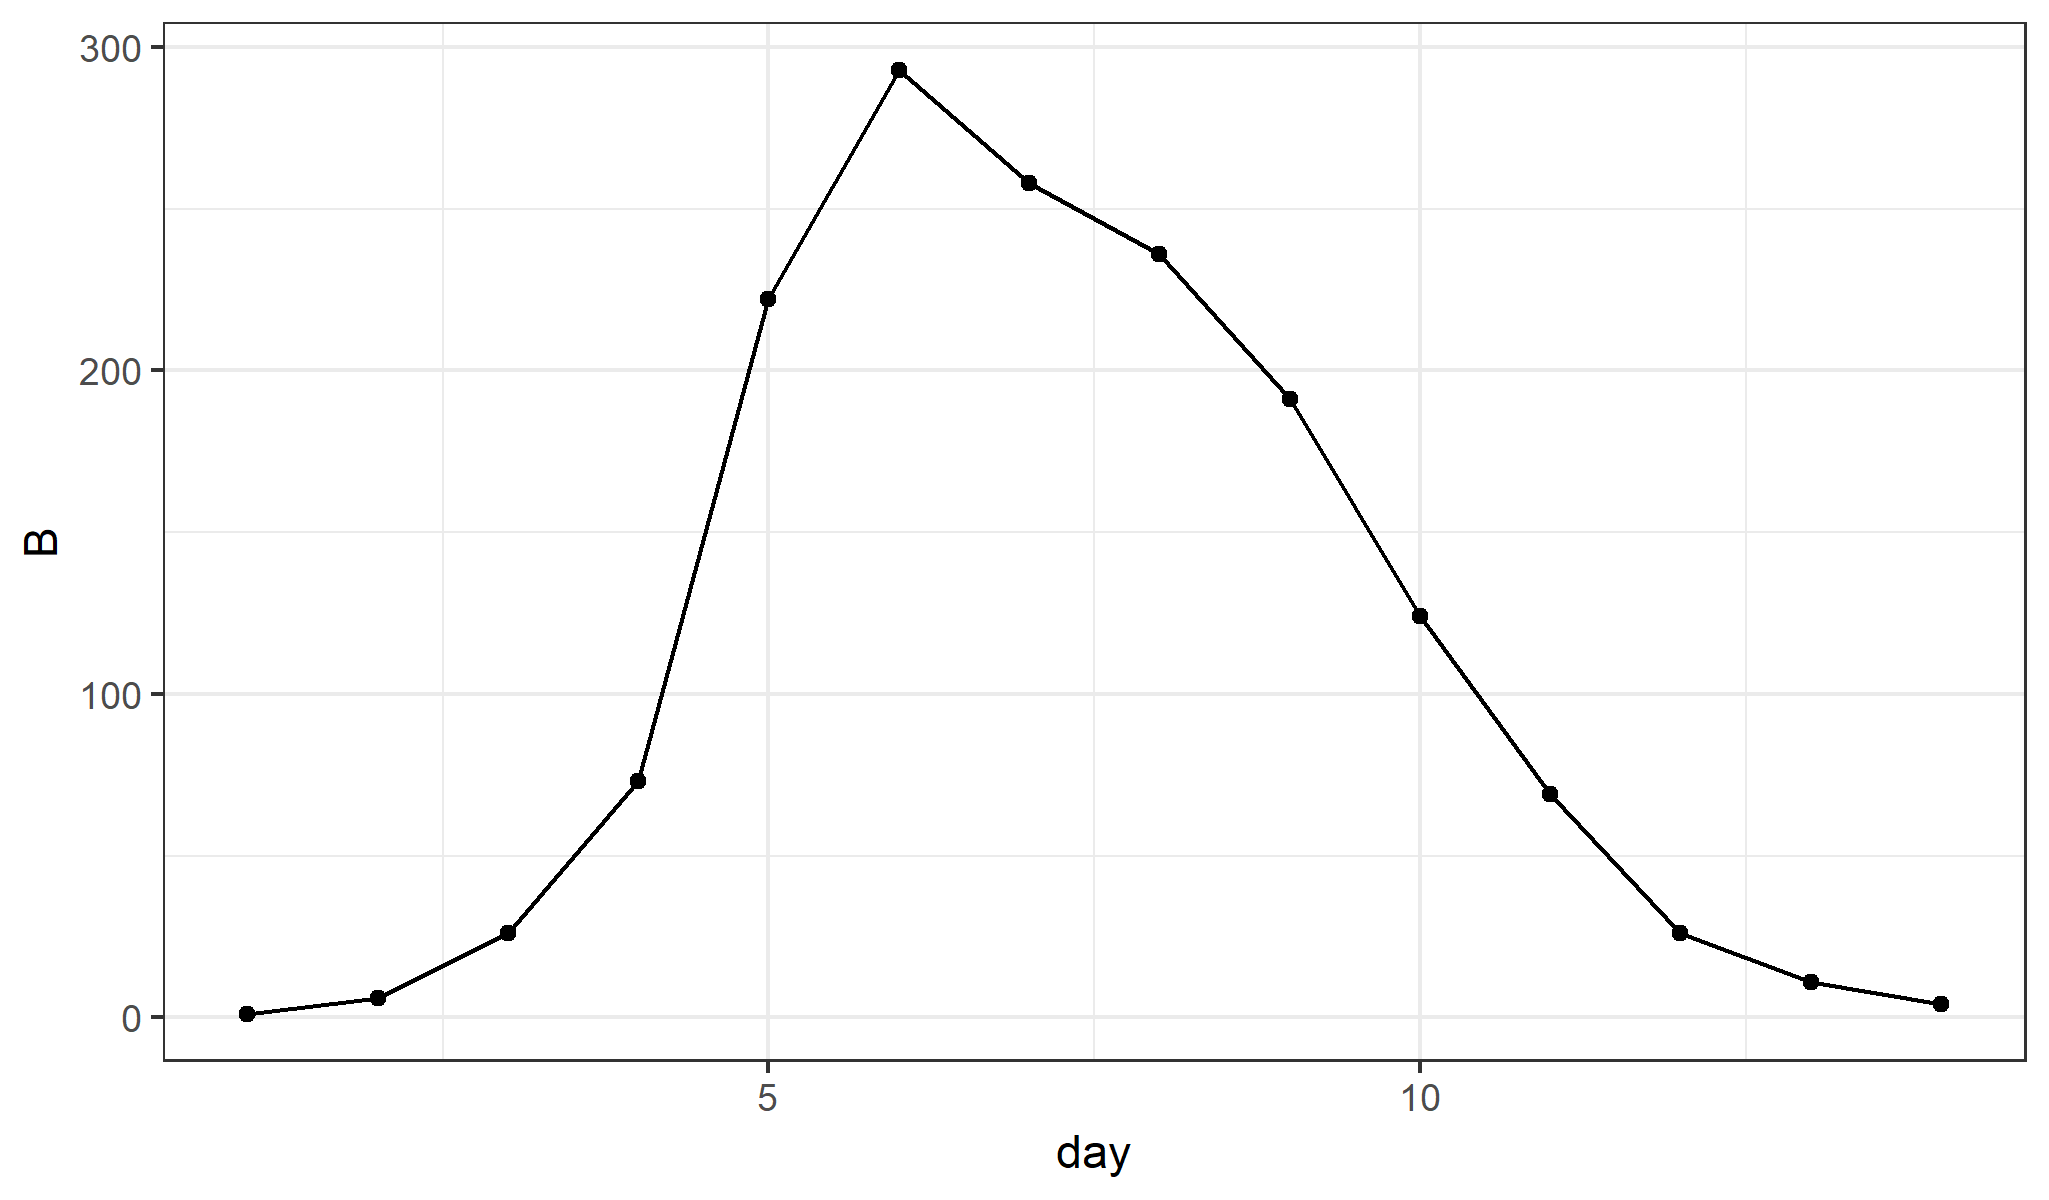
\includegraphics{figure/notes11-flu-data2-1} \end{center}

Let's assume that \(B\) indicates the number of boys confined to bed the
preceding day and that the disease follows the simple SIR model. Our
tasks will be, first, to estimate the parameters of the SIR and, second,
to decide whether or not the SIR model is an adequate description of
these data.

Below is a diagram of the SIR model. The host population is divided into
three classes according to their infection status: S, susceptible hosts;
I, infected (and infectious) hosts; R, recovered and immune hosts. The
rate at which individuals move from S to I is the force of infection,
\(\lambda=\beta\,I/N\), while that at which individuals move into the R
class is \(\gamma\).

\hypertarget{htmlwidget-91698f29ac8403830b98}{}

Let's look at how we can view the SIR as a POMP model. The unobserved
state variables, in this case, are the numbers of individuals, \(S\),
\(I\), \(R\) in the S, I, and R compartments, respectively. It's
reasonable in this case to view the population size \(N=S+I+R\), as
fixed. The numbers that actually move from one compartment to another
over any particular time interval are modeled as stochastic processes.
In this case, we'll assume that the stochasticity is purely demographic,
i.e., that each individual in a compartment at any given time faces the
same risk of exiting the compartment.

To implement the model in \textbf{pomp}, the first thing we need is a
stochastic simulator for the unobserved state process. We've seen that
there are several ways of approximating the process just described for
numerical purposes. An attractive option here is to model the number
moving from one compartment to the next over a very short time interval
as a binomial random variable. \hl{In particular, we model the number,
$\dlta{N_{SI}}$, moving from S to I over interval $\dlta{t}$ as}
\[\dlta{N_{SI}} \sim \dist{Binomial}{S,1-e^{-\lambda\dlta{t}}},\] \hl{and
the number moving from I to R as}
\[\dlta{N_{IR}} \sim \dist{Binomial}{I,1-e^{-\gamma\dlta{t}}}.\]

A \texttt{Csnippet} that encodes such a simulator is as follows:

\begin{Shaded}
\begin{Highlighting}[]
\NormalTok{sir_step <-}\StringTok{ }\KeywordTok{Csnippet}\NormalTok{(}\StringTok{"}
\StringTok{  double dN_SI = rbinom(S,1-exp(-Beta*I/N*dt));}
\StringTok{  double dN_IR = rbinom(I,1-exp(-gamma*dt));}
\StringTok{  S -= dN_SI;}
\StringTok{  I += dN_SI - dN_IR;}
\StringTok{  R += dN_IR;}
\StringTok{"}\NormalTok{)}
\end{Highlighting}
\end{Shaded}

At day zero, we'll assume that \(I=1\) and \(R=0\), but we don't know
how big the school is, so we treat \(N\) as a parameter to be estimated
and let \(S(0)=N-1\). Thus an initializer \texttt{Csnippet} is

\begin{Shaded}
\begin{Highlighting}[]
\NormalTok{sir_init <-}\StringTok{ }\KeywordTok{Csnippet}\NormalTok{(}\StringTok{"}
\StringTok{  S = N-1;}
\StringTok{  I = 1;}
\StringTok{  R = 0;}
\StringTok{"}\NormalTok{)}
\end{Highlighting}
\end{Shaded}

We fold these \texttt{Csnippet}s, with the data, into a \texttt{pomp}
object thus:

\begin{Shaded}
\begin{Highlighting}[]
\KeywordTok{pomp}\NormalTok{(bsflu,}\DataTypeTok{time=}\StringTok{"day"}\NormalTok{,}\DataTypeTok{t0=}\DecValTok{0}\NormalTok{,}\DataTypeTok{rprocess=}\KeywordTok{euler.sim}\NormalTok{(sir_step,}\DataTypeTok{delta.t=}\DecValTok{1}\OperatorTok{/}\DecValTok{6}\NormalTok{),}
     \DataTypeTok{initializer=}\NormalTok{sir_init,}\DataTypeTok{paramnames=}\KeywordTok{c}\NormalTok{(}\StringTok{"N"}\NormalTok{,}\StringTok{"Beta"}\NormalTok{,}\StringTok{"gamma"}\NormalTok{),}
     \DataTypeTok{statenames=}\KeywordTok{c}\NormalTok{(}\StringTok{"S"}\NormalTok{,}\StringTok{"I"}\NormalTok{,}\StringTok{"R"}\NormalTok{)) ->}\StringTok{ }\NormalTok{sir}
\end{Highlighting}
\end{Shaded}

Now let's assume that the case reports, \(B\), result from a process by
which new infections result in confinement with probability \(\rho\),
which we can think of as the probability that an infection is severe
enough to be noticed by the school authorities. Since confined cases
have, presumably, a much lower transmission rate, let's treat \(B\) as
being a count of the number of boys who have moved from I to R over the
course of the past day. We need a variable to track this. Let's modify
our \texttt{Csnippet} above, adding a variable \(H\) to track the
incidence. We'll then replace the \texttt{rprocess} with the new one.

\begin{Shaded}
\begin{Highlighting}[]
\NormalTok{sir_step <-}\StringTok{ }\KeywordTok{Csnippet}\NormalTok{(}\StringTok{"}
\StringTok{  double dN_SI = rbinom(S,1-exp(-Beta*I/N*dt));}
\StringTok{  double dN_IR = rbinom(I,1-exp(-gamma*dt));}
\StringTok{  S -= dN_SI;}
\StringTok{  I += dN_SI - dN_IR;}
\StringTok{  R += dN_IR;}
\StringTok{  H += dN_IR;}
\StringTok{"}\NormalTok{)}

\NormalTok{sir_init <-}\StringTok{ }\KeywordTok{Csnippet}\NormalTok{(}\StringTok{"}
\StringTok{  S = N-1;}
\StringTok{  I = 1;}
\StringTok{  R = 0;}
\StringTok{  H = 0;}
\StringTok{"}\NormalTok{)}

\KeywordTok{pomp}\NormalTok{(sir,}\DataTypeTok{rprocess=}\KeywordTok{euler.sim}\NormalTok{(sir_step,}\DataTypeTok{delta.t=}\DecValTok{1}\OperatorTok{/}\DecValTok{6}\NormalTok{),}\DataTypeTok{initializer=}\NormalTok{sir_init,}
     \DataTypeTok{paramnames=}\KeywordTok{c}\NormalTok{(}\StringTok{"Beta"}\NormalTok{,}\StringTok{"gamma"}\NormalTok{,}\StringTok{"N"}\NormalTok{),}\DataTypeTok{statenames=}\KeywordTok{c}\NormalTok{(}\StringTok{"S"}\NormalTok{,}\StringTok{"I"}\NormalTok{,}\StringTok{"R"}\NormalTok{,}\StringTok{"H"}\NormalTok{)) ->}\StringTok{ }\NormalTok{sir}
\end{Highlighting}
\end{Shaded}

Now, we'll model the data, \(B\), as a binomial process,
\[B_t \sim \dist{Binomial}{H(t)-H(t-1),\rho}.\] But we have a problem,
since at time \(t\), the variable \texttt{H} we've defined will contain
\(H(t)\), not \(H(t)-H(t-1)\). We can overcome this by telling
\texttt{pomp} that we want \texttt{H} to be set to zero immediately
following each observation. We do this by setting the \texttt{zeronames}
argument to \texttt{pomp}:

\begin{Shaded}
\begin{Highlighting}[]
\KeywordTok{pomp}\NormalTok{(sir,}\DataTypeTok{zeronames=}\StringTok{"H"}\NormalTok{) ->}\StringTok{ }\NormalTok{sir}
\end{Highlighting}
\end{Shaded}

Now, to include the observations in the model, we must write both a
\texttt{dmeasure} and an \texttt{rmeasure} component:

\begin{Shaded}
\begin{Highlighting}[]
\NormalTok{dmeas <-}\StringTok{ }\KeywordTok{Csnippet}\NormalTok{(}\StringTok{"lik = dbinom(B,H,rho,give_log);"}\NormalTok{)}
\NormalTok{rmeas <-}\StringTok{ }\KeywordTok{Csnippet}\NormalTok{(}\StringTok{"B = rbinom(H,rho);"}\NormalTok{)}
\end{Highlighting}
\end{Shaded}

and put these into our \texttt{pomp} object:

\begin{Shaded}
\begin{Highlighting}[]
\NormalTok{sir <-}\StringTok{ }\KeywordTok{pomp}\NormalTok{(sir,}\DataTypeTok{rmeasure=}\NormalTok{rmeas,}\DataTypeTok{dmeasure=}\NormalTok{dmeas,}\DataTypeTok{statenames=}\StringTok{"H"}\NormalTok{,}\DataTypeTok{paramnames=}\StringTok{"rho"}\NormalTok{)}
\end{Highlighting}
\end{Shaded}

Let's perform some simulations to verify that things are working. To do
so, we'll need some parameters. A little thought will get us some
ballpark estimates. In the data, it looks like there were a total of
1540 infections, so the population size, \(N\), must be somewhat in
excess of this number. In fact, we can use the final-size equation
\[R_0 = -\frac{\log{(1-f)}}{f},\] where \(f=R(\infty)/N\) is the final
size of the epidemic, together with the idea that \(R_0\) must be, say,
around 1.5, to estimate that \(f\approx 0.6\), whence \(N\approx 2600\).
If the infectious period is roughly 1~da, then
\(1/\gamma \approx 1~\text{da}\) and
\(\beta = \gamma\,R_0 \approx 1.5~\text{da}^{-1}\).

\begin{Shaded}
\begin{Highlighting}[]
\NormalTok{sims <-}\StringTok{ }\KeywordTok{simulate}\NormalTok{(sir,}\DataTypeTok{params=}\KeywordTok{c}\NormalTok{(}\DataTypeTok{Beta=}\FloatTok{1.5}\NormalTok{,}\DataTypeTok{gamma=}\DecValTok{1}\NormalTok{,}\DataTypeTok{rho=}\FloatTok{0.9}\NormalTok{,}\DataTypeTok{N=}\DecValTok{2600}\NormalTok{),}
                 \DataTypeTok{nsim=}\DecValTok{20}\NormalTok{,}\DataTypeTok{as=}\OtherTok{TRUE}\NormalTok{,}\DataTypeTok{include=}\OtherTok{TRUE}\NormalTok{)}

\KeywordTok{ggplot}\NormalTok{(sims,}\DataTypeTok{mapping=}\KeywordTok{aes}\NormalTok{(}\DataTypeTok{x=}\NormalTok{time,}\DataTypeTok{y=}\NormalTok{B,}\DataTypeTok{group=}\NormalTok{sim,}\DataTypeTok{color=}\NormalTok{sim}\OperatorTok{==}\StringTok{"data"}\NormalTok{))}\OperatorTok{+}
\StringTok{  }\KeywordTok{geom_line}\NormalTok{()}\OperatorTok{+}\KeywordTok{guides}\NormalTok{(}\DataTypeTok{color=}\OtherTok{FALSE}\NormalTok{)}
\end{Highlighting}
\end{Shaded}

\begin{center}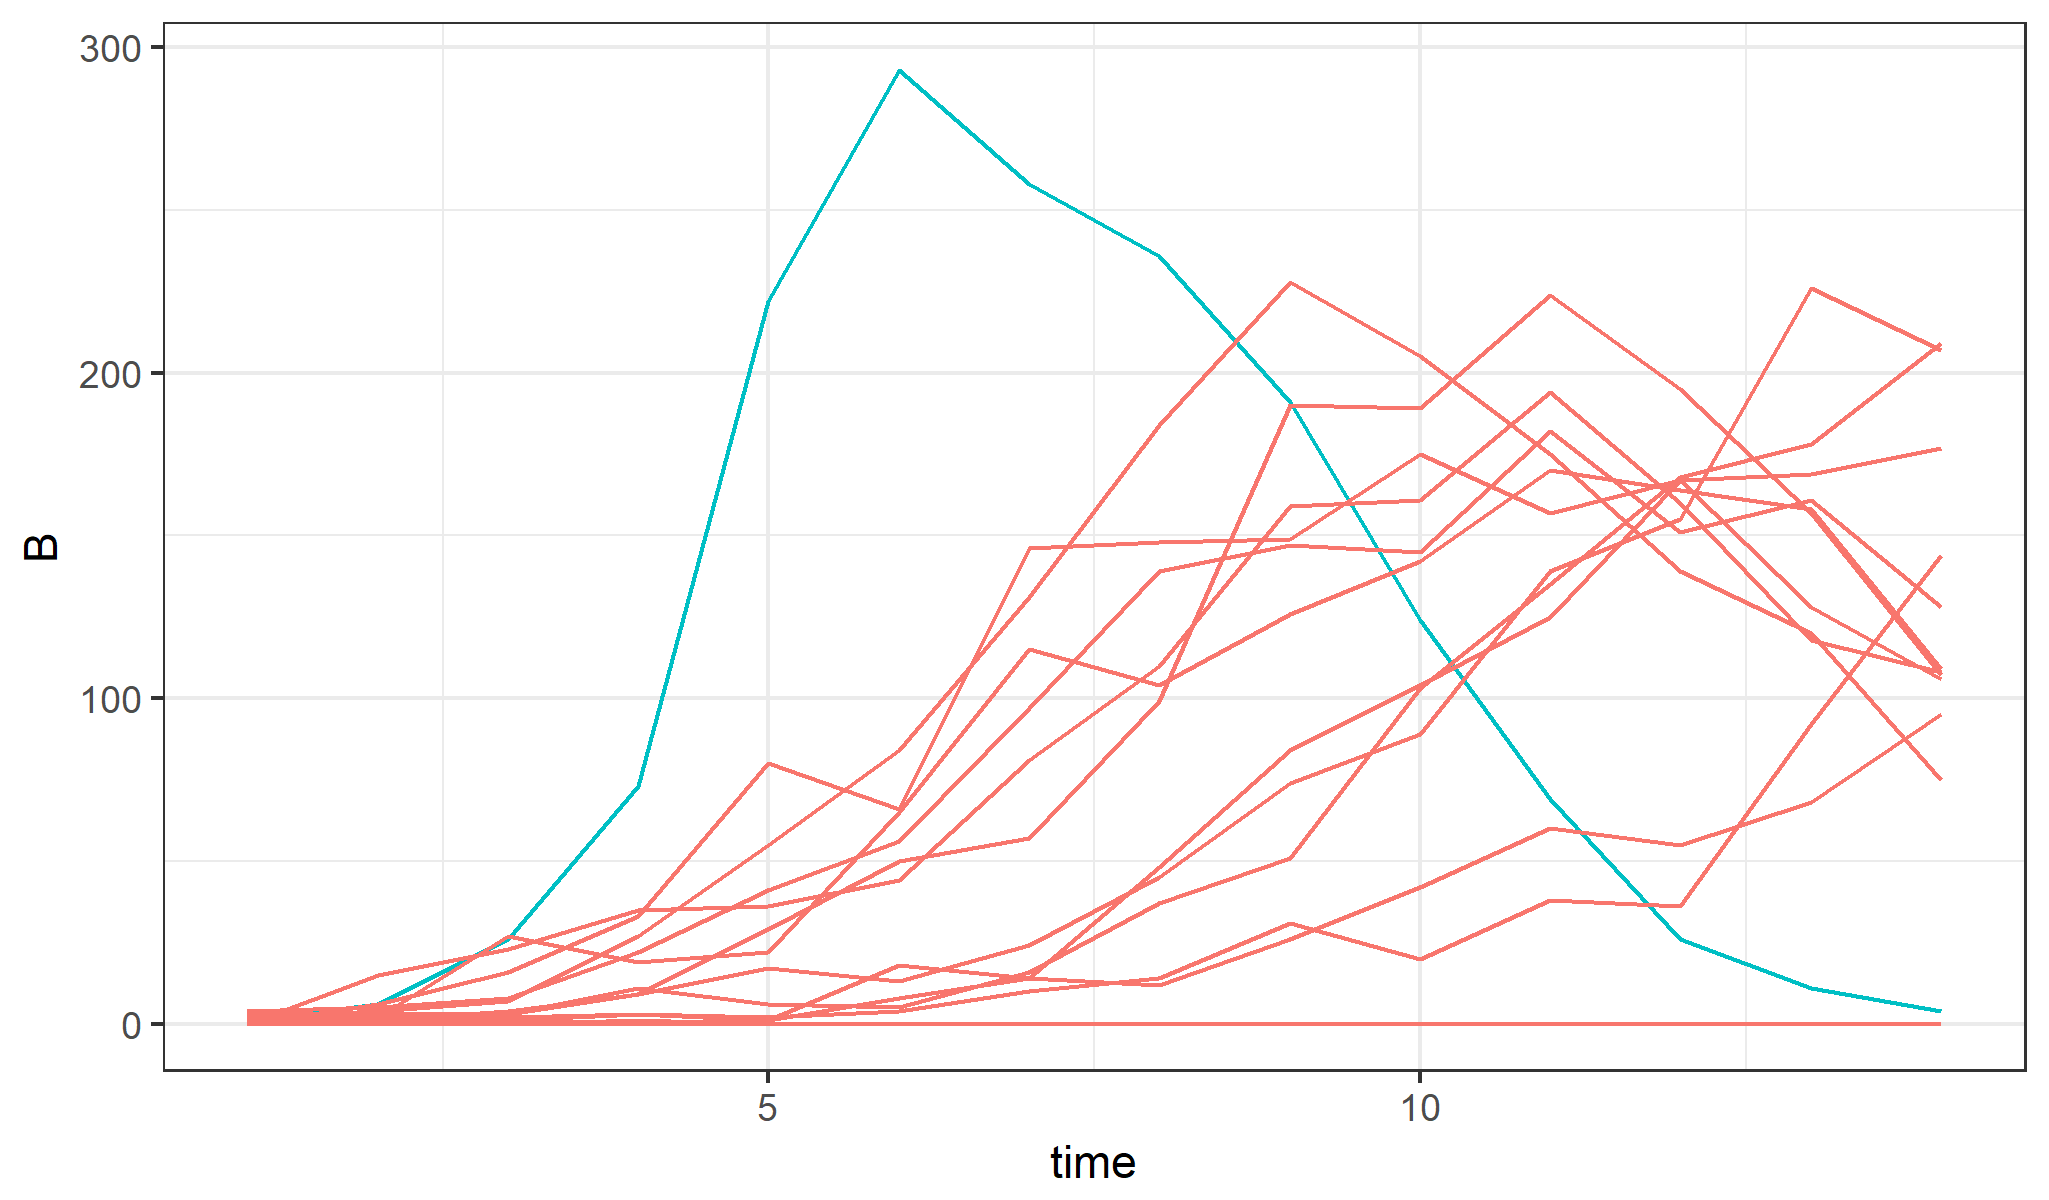
\includegraphics{figure/notes11-unnamed-chunk-1-1} \end{center}

\begin{center}\rule{0.5\linewidth}{\linethickness}\end{center}

\begin{center}\rule{0.5\linewidth}{\linethickness}\end{center}

\subsection{Exercises}\label{exercises-2}

\subsubsection{Explore the SIR model}\label{explore-the-sir-model}

Fiddle with the parameters to see if you can't find parameters for which
the data are a more plausible realization.

\begin{center}\rule{0.5\linewidth}{\linethickness}\end{center}

\begin{center}\rule{0.5\linewidth}{\linethickness}\end{center}

\subsubsection{The SEIR model}\label{the-seir-model}

Below is a diagram of the so-called SEIR model. This differs from the
SIR model in that infected individuals must pass a period of latency
before becoming infectious.

\hypertarget{htmlwidget-eee77e9722f087b30284}{}

Modify the codes above to construct a \texttt{pomp} object containing
the flu data and an SEIR model. Perform simulations as above and adjust
parameters to get a sense of whether improvement is possible by
including a latent period.

\begin{center}\rule{0.5\linewidth}{\linethickness}\end{center}

\begin{center}\rule{0.5\linewidth}{\linethickness}\end{center}

\subsubsection{Rethinking the boarding-school flu
data}\label{rethinking-the-boarding-school-flu-data}

In the preceding, we've been assuming that \(B_t\) represents the number
of boys \emph{sent} to bed on day \(t\). Actually, this isn't correct at
all. As described in the report {[}@anonymous78{]}, \(B_t\) represents
the total number of boys \emph{in} bed on day \(t\). Since boys were
potentially confined for more than one day, the data count each
infection multiple times. On the other hand, we have information about
the total number of boys at risk and the total number who were infected.
In fact, we know from @anonymous78 that \(N=763\) boys were at risk and
\(512\) boys in total spent between 3 and 7 days away from class (either
in bed or convalescent). Moreover, there is information in the data on
the number of boys, \(C_t\), convalescent at day \(t\). Since
\(1540~\text{boy-da}/512~\text{boy} \approx 3~\text{da}\), we know that
the average duration spent in bed was 3~da and, since \(\sum_t\!C_t=0\),
we can infer that the average time spent convalescing was
\(0~\text{boy-da}/512~\text{boy} \approx 0~\text{da}\).

\begin{Shaded}
\begin{Highlighting}[]
\KeywordTok{require}\NormalTok{(reshape2)}
\KeywordTok{ggplot}\NormalTok{(}\DataTypeTok{data=}\KeywordTok{melt}\NormalTok{(bsflu,}\DataTypeTok{id=}\StringTok{"day"}\NormalTok{),}\DataTypeTok{mapping=}\KeywordTok{aes}\NormalTok{(}\DataTypeTok{x=}\NormalTok{day,}\DataTypeTok{y=}\NormalTok{value,}\DataTypeTok{color=}\NormalTok{variable))}\OperatorTok{+}
\StringTok{  }\KeywordTok{geom_line}\NormalTok{()}\OperatorTok{+}\KeywordTok{geom_point}\NormalTok{()}
\end{Highlighting}
\end{Shaded}

\begin{center}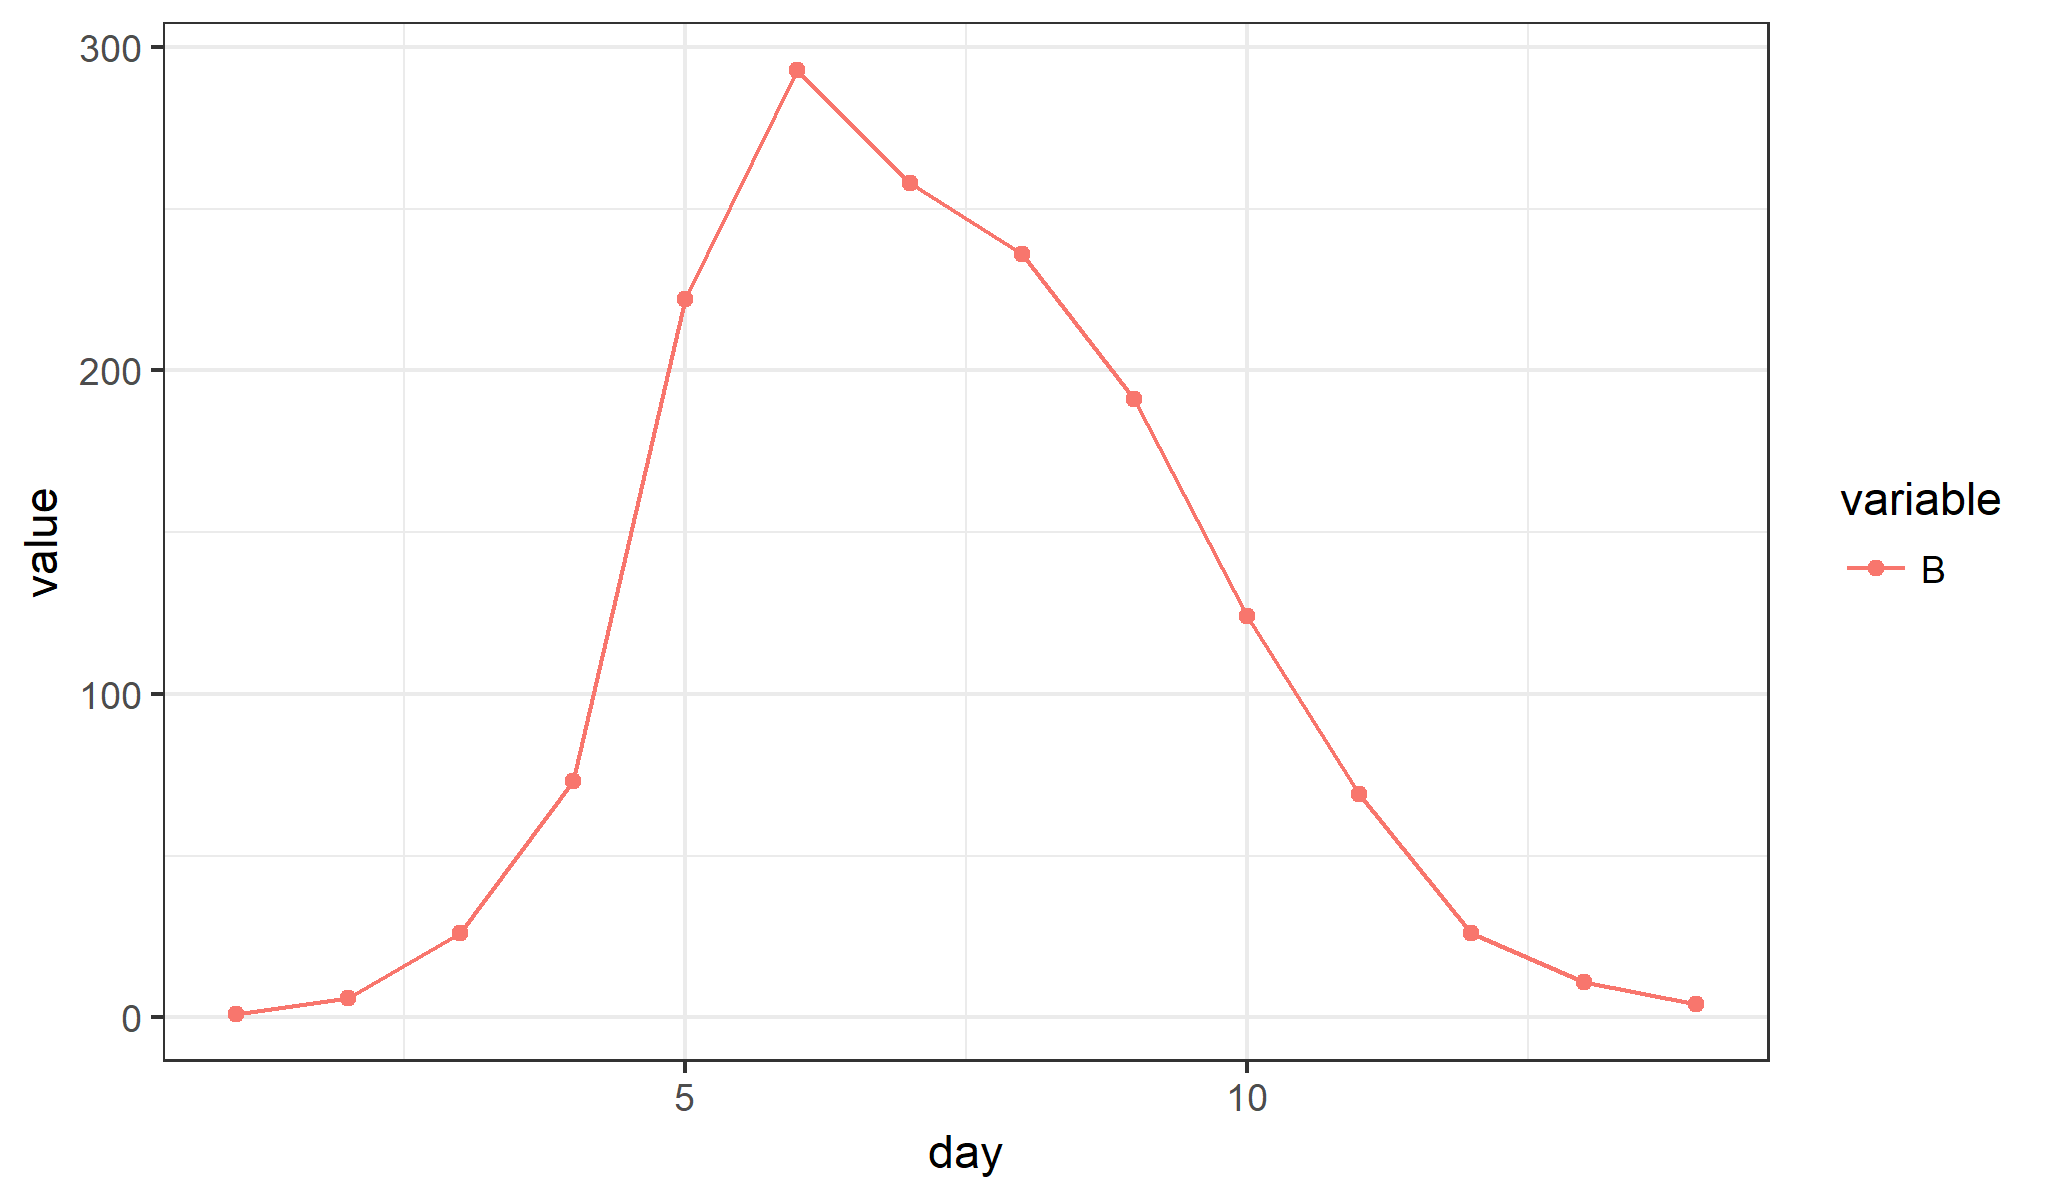
\includegraphics{figure/notes11-bsflu-plot2-1} \end{center}

Formulate a model with both confinement and convalescent stages.
Implement it in \textbf{pomp} using a compartmental model like that
diagrammed below.

$S\longrightarrow I \longrightarrow R1\longrightarrow R2$

\hypertarget{htmlwidget-fcce0d5c6205a6196b75}{}

You will have to give some thought to just how to model the relationship
between the data (\(B\) and \(C\)) and the state variables. How many
parameters can reasonably be fixed? How many must be estimated? Obtain
some ballpark estimates of the parameters and simulate to see if you can
plausibly explain the data as a realization of this model.

\begin{center}\rule{0.5\linewidth}{\linethickness}\end{center}

\begin{center}\rule{0.5\linewidth}{\linethickness}\end{center}

Acknowledgment

These notes were developed from a short course on
\href{http://kingaa.github.io/sbied/}{Simulation-based Inference for
Epidemiological Dynamics} by Aaron King and Edward Ionides, taught at
the University of Washington Summer Institute in Statistics and Modeling
in Infectious Diseases, 2015 to 2017.

\begin{center}\rule{0.5\linewidth}{\linethickness}\end{center}

\subsection*{References}\label{references}
\addcontentsline{toc}{subsection}{References}

\hypertarget{refs}{}
\hypertarget{ref-anonymous78}{}
Anonymous. 1978. Influenza in a boarding school. British Medical Journal
1:587.

\hypertarget{ref-bhadra11}{}
Bhadra, A., E. L. Ionides, K. Laneri, M. Pascual, M. Bouma, and R.
Dhiman. 2011. Malaria in Northwest India: Data analysis via partially
observed stochastic differential equation models driven by Lévy noise.
Journal of the Americal Statistical Association 106:440--451.

\hypertarget{ref-breto09}{}
Bretó, C., D. He, E. L. Ionides, and A. A. King. 2009. Time series
analysis via mechanistic models. Annals of Applied Statistics
3:319--348.

\hypertarget{ref-laneri10}{}
Laneri, K., A. Bhadra, E. L. Ionides, M. Bouma, R. Yadav, R. Dhiman, and
M. Pascual. 2010. Forcing versus feedback: Epidemic malaria and monsoon
rains in NW India. PLoS Comput. Biol. 6:e1000898.


\end{document}
